\documentclass[spanish, fleqn, twocolumn]{IEEEtran/IEEEtran}
\usepackage[spanish]{babel}
\usepackage[utf8]{inputenc}
\usepackage[colorlinks, urlcolor=blue]{hyperref}
\usepackage[top = 2.5cm, bottom = 2cm, left = 2.5cm, right = 2.5cm]{geometry}
\usepackage{fancyhdr, graphicx}
%\usepackage{changepage}
\usepackage{titling}
\usepackage{caption}

\renewcommand\IEEEkeywordsname{Keywords}
\renewcommand{\tt}[1]{\texttt{#1}}
\renewcommand{\bf}[1]{\textbf{#1}}

\renewcommand{\headrulewidth}{0pt}
\fancyhead[L]{\vbox{
\includegraphics[height=2cm]{figures/di} \vspace{0.3cm}}}
\fancyhead[C]{
    \vbox{\textsc{\large Universidad Técnica Federico Santa María}\\[0.14cm]
          \textsc{\LARGE Departamento de Informática} \\[0.14cm]
          \textsc{\Large ICI-309 -- Seminario de Memoria}
\noindent\makebox[\linewidth]{\rule{18cm}{0.5pt}} }}
\fancyhead[R]{\vbox{\includegraphics[height=2cm]{figures/utfsm}\vspace{0.3cm}}}

\title{~\\ Análisis de centralidad a base de datos RDF.\\
       Caso de uso: Datos biológicos.} 
\author{Hernán Vargas Leighton -- 201073009-3 \\ hernan.vargas@alumnos.usm.cl\\~}
\date{\today}

%17:20

\begin{document}
\maketitle
\thispagestyle{empty}
\thispagestyle{fancy}

\section{Definición del problema}
La web como la conocemos está hecha por y para las personas, por lo que las
maquinas actualmente deben emular el comportamiento humano para acceder a
gran cantidad de la información publicada en Internet. Esta problemática intenta
ser solucionada por la web semántica, que entre sus objetivos tiene crear
tecnologías para la publicación y el análisis de los datos en la web por parte
de las computadoras, para ello es necesario crear enlaces y relaciones entre los
datos existentes y ampliar los mismos a todo ámbito de conocimiento.

En este contexto nace Bio2RDF, proyecto que anexa la información de 35 bases de
datos biológicas abiertas a todo publico y crea enlaces entre ellas generando un
total de 11.000 millones de datos enlazados. Para lograrlo utiliza las
tecnologías de la web semántica.

Pero de la gran cantidad de datos que componen el proyecto Bio2RDF no todos
tienen la misma importancia. Actualmente no existen estudios que determinen
cuales son los datos más buscados por parte de los usuarios, es decir, no se
conoce cual es la información más relevante de la base de datos y por ello,
no es posible hacer una optimización teniendo este parámetro en cuenta.

Para determinar la importancia de un dato existen muchas métricas, entre ellas,
el análisis de centralidad que es ideal para este estudio pues podemos modelar
las consultas hechas al proyecto Bio2RDF como un grafo conectado o una red.
La centralidad es uno de los conceptos más estudiados en el análisis de redes,
actualmente se utiliza ampliamente en las redes sociales para determinar las
personas más influyentes.

Así, un análisis de centralidad a los datos consultados por los usuarios del
proyecto Bio2RDF revelará cual es la información más importante para los mismos
y con ello se podrá mejorar el soporte que esta tiene.

\section{Discusión Bibliográfica}
Los datos a analizar en esta memoria serán extraídos del proyecto 
Bio2RDF\cite{callahan2013bio2rdf}\cite{belleau2008bio2rdf}, la
red de datos enlazados más grande de las ciencias naturales. Esta iniciativa se
encuentra en el marco de la web semántica, en un esfuerzo para combinar la
información disponible de diferentes bases de datos abiertas al público general.
Así, se utilizará el conjunto de tecnologías, estándares y recomendaciones
publicadas por la W3C (\emph{World Wide Web Consortium}) para la creación de la
web de datos enlazados.

La web semántica es un conjunto de actividades propuestas por el W3C con el fin
de publicar datos en la web que sean procesables tanto por los usuarios como por
las máquinas. Se basa en la idea de añadir metadatos semánticos y ontológicos
que describan el contenido y las relaciones de los datos publicados. 
Es posible rastrear los orígenes de esta idea hasta una propuesta temprana de la
\emph{world wide web} en 1986 ~\cite{berners1989proposal}.

\begin{figure}[htpb]
  \centering
  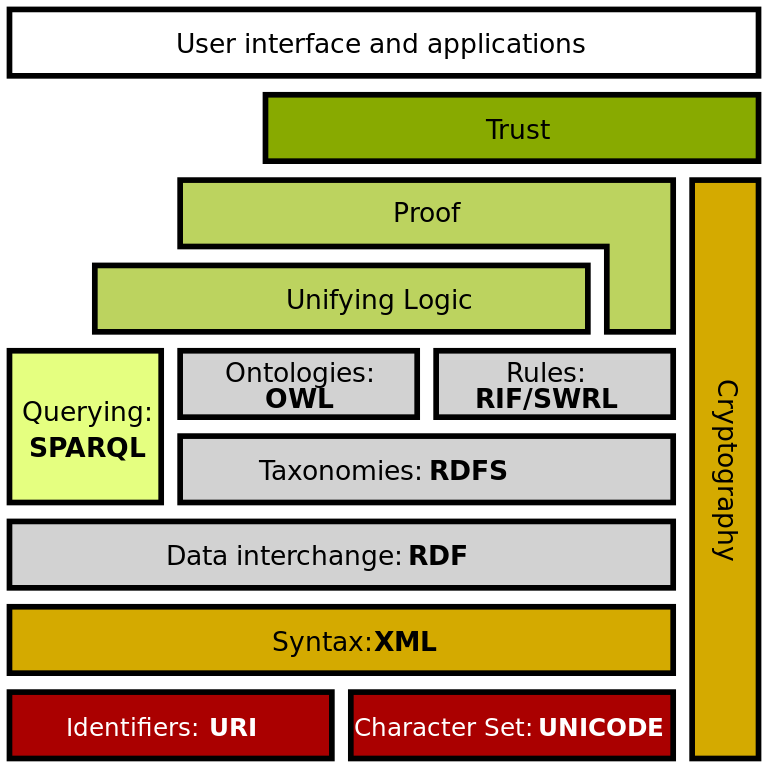
\includegraphics[width=.4\textwidth]{../../trabajos_utfsm/Memoria/Memoria/figures/Semantic_web_stack.png}
  \caption{Pila de tecnologías de la web semántica\cite{wikimg:swstack}.}
  \label{fig:swstack}
\end{figure}

En la figura \ref{fig:swstack} se pueden ver las tecnologías involucradas en la
creación y publicación de datos semánticos en la web. A continuación se hará una
breve revisión de dichas tecnologías.

\newpage
\newgeometry{left=2.5cm, right=2.5cm, top=2.5cm, bottom=2.5cm}

\subsection{Tecnologías del hipertexto}
El componente básico para identificar inequívocamente un recurso en la web se
llama \bf{URI}\cite{berners2004uniform} (\emph{Uniform Resource Identifier}), 
una cadena de caracteres con sintaxis fuertemente estructurada. Cabe destacar
que una URL es una URI que apunta a un recurso físico en la web, mientras que
una URI no necesariamente debe apuntar a una localización que exista realmente.

\bf{XML} (\emph{Extensible Markup Language}) es un
lenguaje de marcas desarrollado por el W3C para almacenar datos de manera
legible tanto por personas como por máquinas. 
El diseño de XML busca la simplicidad, generalidad y usabilidad a través de
internet\cite{paoli2004extensible} lo que lo hace adecuado para representar la
información semántica de los datos. Su extensión XSD (\emph{XML Schema
Definition}) especifica formalmente la estructura y restricciones de los
contenidos de un fichero XML de manera precisa agregando tipos de datos y sus
restricciones\cite{biron2004xml}.

\subsection{Tecnologías de la web semántica}
\bf{RDF} (\emph{Resource Description Framework}) es una familia de
especificaciones del W3C diseñada como un modelo de datos para metadatos.
Fue adoptado como una recomendación del W3C en 1999, mientras que la
especificación 1.0 fue publicada el 2004 y la 1.1 el
2014\cite{bikakis2013semantic}.

El modelo de datos RDF se basa en la idea de hacer declaraciones sobre 
recursos web (URIs) en forma de expresiones $\langle sujeto, predicado, objeto
\rangle$ que son llamados triples RDF.
El $sujeto$ indica el recurso mientras que el $predicado$ denota la relación
con el $objeto$.

Llamaremos vocabulario a la definición de conceptos y relaciones (términos)
utilizados para describir y representar un área de conocimiento.
Otro concepto a tener en cuenta son las ontologías, aunque no existe una clara 
división entre éstas y los vocabularios, generalmente se les considera más
complejas y formales.
En la web semántica una colección de triples RDF puede denotar un vocabulario o
ontología.

Un conjunto de triples RDF será representado naturalmente por un grafo dirigido.
Esta característica faculta la tecnología para ser parte fundamental de la web 
semántica pues permite relacionar información de diferentes fuentes sin mayor
problema y representarla en un esquema fácilmente identificable.

RDF es un modelo abstracto con varios formatos de serialización, por lo que la
codificación de un triple varía dependiendo el tipo de archivo en el que se
guarde. En esta memoria se trabajará con triples codificados en RDF/XML pues
fue fue la primera codificación estándar para serializar RDF (en un archivo
XML).

El vocabulario incluido en la especificación RDF es muy básico y por ello fue
extendido a \emph{RDF Schema}, por lo que la gran mayoría de los \emph{dataset}
RDF contienen ambos vocabularios.

\bf{RDFS} (\emph{Resource Description Framework Schema}) extiende RDF proveyendo
un set de clases y propiedades que mejoran la creación de modelos como son:
\tt{Class} para declarar clases, \tt{subClassOf} para denotar herencia,
\tt{range} y \tt{domain} para el rango y dominio de cierta propiedad
(\tt{rdf:Property}), entre otras.

RDF fue presentado en 1998 e introducido finalmente como recomendación del W3C
el 2004\cite{bikakis2013semantic}. La especificación completa del vocabulario puede encontrarse en ~\cite{brickley2014rdfs}.

\bf{OWL} (\emph{Web Ontology Language}) es una familia de lenguajes para
la creación de ontologías complejas.
Agrega lógica computacional para que las relaciones
hechas con este lenguaje puedan ser procesadas con el fin de verificar la
consistencia de la información o generar información implicita.

La versión actual de OWL se conoce como ``OWL 2'' y fue publicada el 2009 como 
una revisión y extensión de la versión inicial publicada el
2004\cite{bikakis2013semantic}.

OWL 2 tiene tres perfiles dependiendo de la función que cumple.
\begin{enumerate}
  \item \bf{OWL 2 EL}: 
    Es el fragmento del lenguaje decidible en tiempo polinomial, diseñado para
    trabajar con grandes volúmenes de propiedades y clases.
  \item \bf{OWL 2 QL}:
    Fue diseñado para facilitar el acceso a \emph{datasets} con un gran número
    de instancias donde las consultas son más importantes que el razonamiento.
  \item \bf{OWL 2 RL}:
    Está optimizado para el análisis de reglas lógicas, en aplicaciones que
    requieren un razonamiento escalable sin perder la expresividad del lenguaje.
\end{enumerate}
Se pueden ver las características completas de los perfiles de OWL 2 en
~\cite{motik2009owlprofiles}.

\bf{SPARQL} (\emph{SPARQL Protocol and RDF Query Language}) es un lenguaje
estandarizado para consultar grafos RDF, se constituyó como una recomendación
oficial por la W3C en el 2008\cite{bikakis2013semantic}. La versión actual de
SPARQL es la 1.1\cite{world2013sparql}.

SPARQL provee un set completo de operaciones analíticas para sus consultas
definidas directamente en la especificación. Particularmente provee 4 formas de
consultas:
\begin{itemize}
  \item \bf{\tt{SELECT}}:
    Retorna valores en forma de tabla.
  \item \bf{\tt{CONSTRUCT}}:
    Retorna valores en forma de triple RDF.
  \item \bf{\tt{ASK}}:
    Retorna un resultado binario a la consulta (\tt{True/False}).
  \item \bf{\tt{DESCRIBE}}:
    Retorna un grafo RDF con contenido que el administrador del \emph{endpoint}
    SPARQL considere información útil.
\end{itemize}
A excepción de \tt{DESCRIBE}, las demás consultas necesitan un bloque \tt{WHERE}
para determinar las restricciones de búsqueda.

Una descripción completa del lenguaje puede
encontrarse en ~\cite{prud2008sparql} y en ~\cite{world2013sparql}.

\subsection{Centralidad}
La centralidad en un grafo se refiere a una medida de importancia relativa de un
nodo dentro de éste.\cite{borgatti2005centrality}

Conocer la centralidad de un nodo ayuda a determinar, por ejemplo, el impacto
de una persona en una red social, la importancia de una carretera en una red
urbana, los componentes esenciales de una red de computadoras, entre otros.

El concepto fue introducido a fines de los años 1940 por Alex
Bavelas\cite{bavelas1948mathematical}
Es uno de los conceptos más estudiados en el análisis de redes y desde finales
de los años 70 se ha ampliado su uso a las redes
sociales\cite{freeman1979centrality}

Desde sus inicios se han propuesto diversas medidas para determinar la
centralidad de un nodo. Las siguientes son las más utilizadas en análisis de
redes:
\begin{itemize}
  \item La centralidad de grado (\emph{degree centrality})
  \item La cercanía (\emph{closeness})
  \item La intermediación (\emph{betweenness})
  \item La centralidad de vector propio (\emph{eigenvector centrality}).
\end{itemize}

El conocido algoritmo PageRank de Google para determinar la importancia de una
página web es una modificación de un algoritmo de centralidad de vector propio.

\section{Objetivos}
\subsection{Objetivo General}
Generar estadísticas de centralidad sobre el subconjunto de datos consultados
por los usuarios al proyecto Bio2RDF.

\subsection{Objetivos Específicos}
Para el logro del objetivo general se plantean los siguientes objetivos
específicos:
\begin{enumerate}
  \item
    Generar un subgrafo del proyecto Bio2RDF a través del análisis de las
    consultas SPARQL hechas al servidor por parte de los usuarios.
  \item
    Analizar el grafo generado por medio de métricas de centralidad para grafos.
  \item
    Comparar los resultados del estudio con el proyecto Bio2RDF.
\end{enumerate}

\section{Plan de trabajo}
\begin{table}[htpb]
  \centering
  \begin{tabular}{|l|c|}
    \hline %TODO
    \textbf{Actividad} & \textbf{Semanas} \\ \hline
    Elaboración de Estado del Arte & 8 \\
    Extracción de consultas SPARQL de los usuarios & 1 \\
    Modificación de consultas para crear triples RDF & 1 \\
    Creación del grafo consultado por los usuarios & 2 \\
    \begin{tabular}{@{}l@{}}
      Implementación de algoritmos para calcular métricas \\
      de centralidad a grafos RDF
    \end{tabular} & 2 \\
    Calculo de centralidad sobre el grafo de consultas & 2 \\
    Análisis de resultados & 2 \\
    Redacción del Informe Final & 4 \\
    Revisión y Correcciones & 2 \\ \hline
    \textbf{Total} & 24 \\ \hline
  \end{tabular}
\end{table}

\renewcommand{\refname}{\selectfont Referencias} % Hack para nombre
\bibliographystyle{ieeetr}
\bibliography{../../trabajos_utfsm/Memoria/Memoria/Bibliografia/bibliografia,../../trabajos_utfsm/Memoria/Memoria/Bibliografia/W3C,../../trabajos_utfsm/Memoria/Memoria/Bibliografia/images}

%Tiempo SCT
\section*{Tiempo SCT:}
\begin{table}[htpb]
  \centering
  \begin{tabular}{|l|c|}
    \hline %TODO
    \textbf{Actividad} & \textbf{Horas} \\ \hline
    Investigación\footnotemark & 26:00 \\
    Plan de trabajo & 01:00 \\
    Creación de informe & 04:30 \\ \hline
    \textbf{Total} & 27:30 \\ \hline
  \end{tabular}
\end{table}

\footnotetext{Incluida parte de la investigación hecha para otros entregables.}

\end{document}
